\chapter{System Architecture}
\label{ch:system_architecture}

\section{Overview}

The Bitcoin ML Pipeline is designed as a modular, scalable system with clear separation of concerns. This chapter presents the overall architecture and component interactions.

\section{High-Level Architecture Diagram}

\begin{figure}[H]
\centering
\begin{tikzpicture}[scale=1.0, node distance=2cm]
    % Layer 1: Data Sources
    \node[draw, rounded rectangle, fill=blue!20, minimum width=3cm] (coingecko) at (0, 10) {CoinGecko API};
    \node[draw, rounded rectangle, fill=blue!20, minimum width=3cm] (alphavantage) at (4, 10) {Alpha Vantage};
    
    % Layer 2: Data Pipeline
    \node[draw, rectangle, fill=green!20, minimum width=4cm, minimum height=1cm] (fetch) at (2, 8) {Data Fetching \& Validation};
    \node[draw, rectangle, fill=green!20, minimum width=4cm, minimum height=1cm] (preprocess) at (2, 6) {Preprocessing \& Feature Engineering};
    
    % Layer 3: Feature Store
    \node[draw, rounded rectangle, fill=yellow!20, minimum width=3cm] (hopsworks) at (2, 4) {Feature Store (Hopsworks)};
    
    % Layer 4: Model Training
    \node[draw, rectangle, fill=orange!20, minimum width=3.5cm, minimum height=1cm] (training) at (2, 2) {Model Training \& Evaluation};
    
    % Layer 5: Model Registry
    \node[draw, rounded rectangle, fill=purple!20, minimum width=3cm] (registry) at (2, 0) {Model Registry};
    
    % Layer 6: Serving
    \node[draw, rectangle, fill=red!20, minimum width=2cm, minimum height=0.8cm] (api) at (0.5, -2) {FastAPI};
    \node[draw, rectangle, fill=red!20, minimum width=2cm, minimum height=0.8cm] (dashboard) at (3.5, -2) {Streamlit};
    
    % Layer 7: Deployment
    \node[draw, rounded rectangle, fill=gray!20, minimum width=3.5cm, minimum height=0.8cm] (docker) at (2, -3.5) {Docker Containers};
    
    % Arrows
    \draw[->] (coingecko) -- (fetch);
    \draw[->] (alphavantage) -- (fetch);
    \draw[->] (fetch) -- (preprocess);
    \draw[->] (preprocess) -- (hopsworks);
    \draw[->] (hopsworks) -- (training);
    \draw[->] (training) -- (registry);
    \draw[->] (registry) -- (api);
    \draw[->] (registry) -- (dashboard);
    \draw[->] (api) -- (docker);
    \draw[->] (dashboard) -- (docker);
\end{tikzpicture}
\caption{Bitcoin ML Pipeline - High-Level Architecture}
\label{fig:architecture_high_level}
\end{figure}

\section{Component Details}

\subsection{1. Data Ingestion Layer}

\subsubsection{Data Sources}
\begin{itemize}
    \item \textbf{CoinGecko API}: Free, no rate limits, provides OHLCV data + market cap + volume
    \item \textbf{Alpha Vantage}: Paid tier, alternative with similar data
\end{itemize}

\subsubsection{Responsibilities}
\begin{enumerate}
    \item Fetch latest Bitcoin data (hourly via CI/CD)
    \item Validate data quality (non-null, correct types)
    \item Handle API failures gracefully
    \item Store raw data to CSV/database
\end{enumerate}

\textbf{Key Files:}
\begin{itemize}
    \item `src/fetch\_bitcoin\_data.py` (180+ lines)
    \item `src/fetch\_alpha\_vantage.py` (192 lines)
\end{itemize}

\subsection{2. Preprocessing \& Feature Engineering Layer}

\textbf{Input:} Raw OHLCV data  
\textbf{Output:} 24 normalized technical indicators

\begin{equation}
X_{raw} \xrightarrow{\text{Clean}} X_{clean} \xrightarrow{\text{Engineer}} X_{features} \xrightarrow{\text{Normalize}} X_{normalized}
\end{equation}

\subsubsection{Processing Steps}
\begin{enumerate}
    \item \textbf{Data Cleaning:} Missing value imputation, outlier detection
    \item \textbf{Feature Engineering:} Calculate 24 technical indicators
    \item \textbf{Normalization:} StandardScaler (zero mean, unit variance)
    \item \textbf{Temporal Validation:} Ensure proper time ordering
\end{enumerate}

\textbf{Key Files:}
\begin{itemize}
    \item `src/preprocess\_bitcoin.py` (200+ lines)
    \item `src/feature\_engineering.py` (200+ lines)
\end{itemize}

\subsection{3. Feature Store Layer}

\textbf{Technology:} Hopsworks (free tier)

\textbf{Purpose:}
\begin{itemize}
    \item Centralized feature management
    \item Feature versioning and lineage
    \item Online/offline feature serving
    \item Automatic drift detection
\end{itemize}

\textbf{Components:}
\begin{itemize}
    \item \textbf{Feature Group:} `bitcoin\_features` (24 features)
    \item \textbf{Feature View:} `bitcoin\_training\_view` (point-in-time correct)
    \item \textbf{Inference View:} `bitcoin\_inference\_view` (for serving)
\end{itemize}

\textbf{Key Files:}
\begin{itemize}
    \item `src/feature\_store.py` (500+ lines)
    \item `scripts/ingest\_features.py` (200+ lines)
\end{itemize}

\subsection{4. Model Training Layer}

\textbf{Input:} Features from Feature Store  
\textbf{Output:} Trained classification \& regression models

\subsubsection{Models Trained}
\begin{itemize}
    \item \textbf{Classification:} Random Forest (70\% accuracy)
    \item \textbf{Regression:} XGBoost (RMSE 2.8)
    \item \textbf{Ensemble:} Combined classification + regression
\end{itemize}

\subsubsection{Training Pipeline}
\begin{enumerate}
    \item Fetch features from Feature Store
    \item Create classification target (UP/DOWN)
    \item Create regression target (price change \%)
    \item Split temporally (80/20)
    \item Train classification model
    \item Train regression model
    \item Evaluate both on test set
    \item Version models in registry
\end{enumerate}

\textbf{Key Files:}
\begin{itemize}
    \item `src/train\_with\_feature\_store.py` (400+ lines)
    \item `src/train\_all\_models.py` (560+ lines)
    \item `src/model\_experiments.py` (300+ lines)
\end{itemize}

\subsection{5. Model Registry}

\textbf{Storage:} File-based registry in `models/manifest.json`

\textbf{Tracks:}
\begin{itemize}
    \item Model artifacts (.pkl files)
    \item Feature columns (.json)
    \item Training metadata (metrics, date, version)
    \item Model lineage and history
\end{itemize}

\textbf{Example:}
\begin{lstlisting}[language=json]
{
  "active_version": "v20251205T052715Z",
  "versions": {
    "v20251205T052715Z": {
      "clf_model": "models/v20251205T052715Z_clf_model.pkl",
      "reg_model": "models/v20251205T052715Z_reg_model.pkl",
      "created_at": "2025-12-05T07:27:15Z",
      "metrics": {...}
    }
  }
}
\end{lstlisting}

\subsection{6. Serving Layer}

\subsubsection{FastAPI Backend}
\begin{itemize}
    \item \textbf{Port:} 8000 (default)
    \item \textbf{Endpoints:}
    \begin{itemize}
        \item `GET /` — Health check
        \item `GET /model-info` — Model metadata
        \item `POST /predict/classification` — Predict price direction
        \item `POST /predict/regression` — Predict price change \%
    \end{itemize}
    \item \textbf{Response Time:} < 100ms
\end{itemize}

\textbf{Key Files:}
\begin{itemize}
    \item `api/main.py` (300+ lines)
    \item `api\_server.py` (500+ lines)
\end{itemize}

\subsubsection{Streamlit Dashboard}
\begin{itemize}
    \item \textbf{Port:} 8501 (default)
    \item \textbf{Features:}
    \begin{itemize}
        \item Real-time price prediction
        \item Interactive charts (Plotly)
        \item Technical indicators display
        \item Model performance metrics
        \item Feature importance ranking
    \end{itemize}
\end{itemize}

\textbf{Key Files:}
\begin{itemize}
    \item `app.py` (448 lines)
\end{itemize}

\subsection{7. Orchestration Layer}

\subsubsection{Prefect Workflows}
\begin{itemize}
    \item Orchestrates entire ML pipeline
    \item Handles task dependencies
    \item Provides error handling \& retries
    \item Logs all executions
\end{itemize}

\textbf{Key Files:}
\begin{itemize}
    \item `prefect/flows/ml\_pipeline.py` (700+ lines)
\end{itemize}

\subsubsection{GitHub Actions}
\begin{itemize}
    \item Triggers data fetch (hourly)
    \item Triggers training (daily)
    \item Runs CI/CD checks
    \item Manages model versioning
\end{itemize}

\section{Data Flow Diagram}

\begin{figure}[H]
\centering
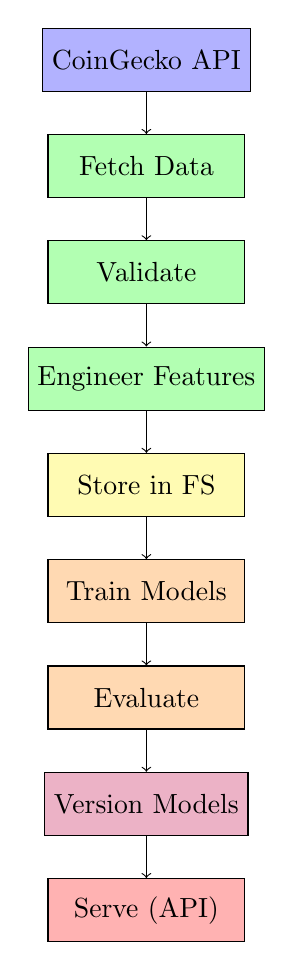
\begin{tikzpicture}[scale=0.9, node distance=2.5cm]
    \node[draw, fill=blue!30, minimum width=2.5cm, minimum height=0.8cm] (1) at (0, 10) {CoinGecko API};
    \node[draw, fill=green!30, minimum width=2.5cm, minimum height=0.8cm] (2) at (0, 8.5) {Fetch Data};
    \node[draw, fill=green!30, minimum width=2.5cm, minimum height=0.8cm] (3) at (0, 7) {Validate};
    \node[draw, fill=green!30, minimum width=2.5cm, minimum height=0.8cm] (4) at (0, 5.5) {Engineer Features};
    \node[draw, fill=yellow!30, minimum width=2.5cm, minimum height=0.8cm] (5) at (0, 4) {Store in FS};
    \node[draw, fill=orange!30, minimum width=2.5cm, minimum height=0.8cm] (6) at (0, 2.5) {Train Models};
    \node[draw, fill=orange!30, minimum width=2.5cm, minimum height=0.8cm] (7) at (0, 1) {Evaluate};
    \node[draw, fill=purple!30, minimum width=2.5cm, minimum height=0.8cm] (8) at (0, -0.5) {Version Models};
    \node[draw, fill=red!30, minimum width=2.5cm, minimum height=0.8cm] (9) at (0, -2) {Serve (API)};
    
    \draw[->] (1) -- (2);
    \draw[->] (2) -- (3);
    \draw[->] (3) -- (4);
    \draw[->] (4) -- (5);
    \draw[->] (5) -- (6);
    \draw[->] (6) -- (7);
    \draw[->] (7) -- (8);
    \draw[->] (8) -- (9);
\end{tikzpicture}
\caption{Data and Model Flow Through Pipeline}
\label{fig:data_flow}
\end{figure}

\section{Scalability Considerations}

\subsection{Horizontal Scaling}
\begin{itemize}
    \item \textbf{Multiple API replicas:} Load balanced via nginx
    \item \textbf{Distributed training:} Support for multi-GPU via TensorFlow Distributed
    \item \textbf{Distributed feature store:} Hopsworks supports enterprise clusters
\end{itemize}

\subsection{Vertical Scaling}
\begin{itemize}
    \item \textbf{Larger models:} LSTM with more layers
    \item \textbf{More data:} Currently 5,600+ records; can scale to millions
    \item \textbf{Richer features:} Can add on-chain metrics, sentiment analysis
\end{itemize}

\section{Monitoring \& Observability}

\subsection{Metrics Tracked}
\begin{itemize}
    \item Model accuracy \& F1-score
    \item Prediction latency
    \item API availability (uptime)
    \item Data drift (feature distributions)
    \item Model drift (performance degradation)
\end{itemize}

\subsection{Logging}
\begin{itemize}
    \item Prefect task logs (structured)
    \item API request logs
    \item Error stacks (sent to Discord)
    \item Training metrics (JSON format)
\end{itemize}

\subsection{Alerting}
\begin{itemize}
    \item Discord webhooks for failures
    \item Performance degradation alerts
    \item Data drift detection
    \item API downtime alerts
\end{itemize}

\section{Summary}

The architecture is modular, scalable, and production-ready:
\begin{itemize}
    \item ✅ Clear separation of concerns
    \item ✅ Extensible design (easy to add new models)
    \item ✅ Containerized for cloud deployment
    \item ✅ Observable (comprehensive logging)
    \item ✅ Resilient (error handling, retries)
\end{itemize}

